\documentclass{article}
\usepackage[english,russian]{babel}
\usepackage[14pt]{extsizes}
\usepackage[left=3cm,right=2cm,top=2cm,bottom=2cm,bindingoffset=0cm]{geometry}
\linespread{1.3}
\usepackage[dvips]{graphicx}
\graphicspath{{./img/}}
\usepackage{color}
\usepackage[colorlinks,linkcolor=blue,urlcolor=blue]{hyperref}
\usepackage[indentfirst]{titlesec}
\usepackage{titletoc}
\usepackage{ltxtable}
\usepackage{xcolor}

\usepackage[utf8]{inputenc}
\setcounter{tocdepth}{3}
\author{Шаймарданов123 Р. Р.}
\begin{document}

\begin{titlepage}
	\begin{center}
		{\large\textsc{Университет ИТМО}}
		\vskip 1pt \hrule \vskip 3pt
		{\large\textsc{Кафедра вычислительной техники}}
		\vfill
		{\LargeОтчет по прохождению практики\vskip 12pt\bfseries Параллельные вычисления}	
	\end{center}
	\vfill	
	\begin{flushright}
		{Выполнил студент\\группы P3310\\Шаймарданов Р.\,Р.\vskip 12pt Руководитель\\Соснин В.\,В.}
	\end{flushright}	
	\vfill	
	\begin{center}
		Санкт-Петербург\\2016
	\end{center}
\end{titlepage}

\tableofcontents
\newpage

\section{Введение}
	\textbf{Цель:} составить составить список из наиболее авторитетных литературных источников по "Параллельным вычислениям".\\
	
	\textbf{Задачи}
	\begin{enumerate}
		\item Описать инструментарий, необходимый для выполнения практического задания.
   		\item Составить перечень современных (новее 2010 года) англоязычных источников, посвящённых параллельным вычислениям в системах с общей памятью.
   		\item Разбить найденные источники на четыре группы: 
   			\begin{itemize}
   		   		\item платные книги 
   		   		\item журналы 
   		   		\item бесплатные книги
   		   		\item онлайн-курсы
   		   	\end{itemize}
   		\item Сформулировать критерий уровня авторитетности для найденных материалов, выполнить ранжирование источников внутри групп.
   		\item Найти, провести разбиение и ранжировать русскоязычные источники, аналогично с иностранными. 
   		\item Провести сравнение работы потоков при различных запусках ОС.
	\end{enumerate}
\newpage

\section{Инструментарий}	
	\subsection{Система компьютерной верстки \TeX(\LaTeX)}
		\subsubsection{Описание}
	\TeX "--- это низкоуровневый язык разметки и программирования, созданный Дональдом Кнутом для единообразной вёрстки документов. Кнут начал разрабатывать систему набора текста \TeX в 1977 году для исследования потенциальных возможностей оборудования цифровой печати, которое в то время начинало проникать в издательское дело. Главным образом он надеялся улучшить качество печатной продукции, которое расстраивало в его собственных книгах и статьях. После выпуска в 1989 году поддержки восьмибитных символов разработка \TeX приостановилась, только иногда выходили версии с исправленными ошибками.\\

	\LaTeX  "--- основанный на \TeX пакет макросов, созданный Лесли Лампортом. Основная цель "--- упростить вёрстку текста, особенно в документах с математическими формулами. Значительно позднее авторы разработали для \LaTeX расширения, которые называются пакетами или стилями. Некоторые из них распространяются вместе с большинством дистрибутивов \TeX/\LaTeX.\\

	Так как \LaTeX содержит часть команд \TeX, то создание документа в \LaTeX - тоже программирование: создаётся текстовый файл в \LaTeX разметке, макросы LaTeX обрабатывают его и производят конечный документ.\\
		\subsubsection{Сравнение с другими программными средствами}
	Подход \LaTeX к созданию документа называется WYSIWYM\footnote{What You See Is What You Mean (То, что ты видишь, есть то, что ты имеешь в виду)}: во время набора текста Вы не видите окончательный вариант документа, только логическую структуру этого документа. Оформлением занимается сам \LaTeX. Такой подход имеет как достоинства, так и недостатки по сравнению с WYSIWYG\footnote{What You See Is What You Get (Что видишь, то и получишь)} программами, такими как Openoffice.org Writer или Microsoft Word.\\
	\textit{Достоинства:}
	\begin{itemize}
   		\item Файлы с исходными текстами можно просмотреть в любом текстовом редакторе, они понятнее в отличие от сложных бинарных файлов и форматов XML, используемых WYSIWYG программами.
   		\item Вы полностью сосредотачиваетесь на структуре и содержании документа и забываете о том, как будет выглядеть печатный вариант.
   		\item Легко скопировать структуру документа в другой документ, в WYSIWYG программах не всегда ясно, какое именно было использовано форматирование.
   		\item Так как исходный документ содержит просто текст, с помощью программных средств на любом языке программирования можно создать таблицы, рисунки, формулы и т.д.
	\end{itemize}	
	\textit{Недостатки:}
	\begin{itemize}
		\item Во время редактирования документа нельзя (обычно) увидеть его окончательный вариант без компиляции.
   		\item Необходимо знать нужные команды разметки \LaTeX.
   		\item Иногда сложно получить требуемый вид документа.
	\end{itemize}
	Документ \LaTeX "--- обычный текстовый файл, в котором указано содержание документа вместе с дополнительной разметкой. При обработке исходного файла макросами \LaTeX можно получить документ в разных форматах. Изначально \LaTeX поддерживает форматы DVI и PDF, но при использовании другого ПО можно легко получить PostScript, PNG, JPG и т.д.

		\subsubsection{Выбор инструмента редактирования}
			В ходе изучения всех возможных вариантов работа с \LaTeX ~для создания данного отчета, была выбрана программа Textmaker
			
			Выбор Textmaker'а обусловлен следующими его особенностями:
			\begin{itemize} 
	    		\item	Автоматическая подсветка синтаксиса
	    		\item	Функция автодополнения команд \LaTeX
	    		\item	Сокрытие блоков кода 
	    		\item	Быстрая навигация по структуре документа
	    		\item	Указание на строку с ошибкой, для быстрой отладки
	    		\item	Интегрированный просмотр PDF
			\end{itemize} 
	\newpage
	\subsection{Система контроля версий Git}
		\subsubsection{Описание}
		Система управления версиями "--- программное обеспечение для облегчения работы с изменяющейся информацией. Система управления версиями позволяет хранить несколько версий одного и того же документа, при необходимости возвращаться к более ранним версиям, определять, кто и когда сделал то или иное изменение, и многое другое.\\
		
		Git "--- это гибкая, распределённая система управления версиями. Проект был создан Линусом Торвальдсом для управления разработкой ядра Linux, первая версия выпущена 7 апреля 2005 года. На сегодняшний день его поддерживает Джунио Хамано. Программа является свободной и выпущена под лицензией GNU GPL версии 2.\\ 
		
	У каждого разработчика, использующего Git, есть свой локальный репозиторий, позволяющий локально управлять версиями. Затем, сохраненными в локальный репозиторий данными, можно обмениваться с другими пользователями. Часто при работе с Git создают центральный репозиторий, с которым остальные разработчики синхронизируются. В этом случае все участники проекта ведут свои локальны разработки и беспрепятственно скачивают обновления из центрального репозитория. Когда необходимые работы отдельными участниками проекта выполнены и отлажены, они, после удостоверения владельцем центрального репозитория в корректности и актуальности проделанной работы, загружают свои изменения в центральный репозиторий. Работа над версиями проекта в Git может вестись в нескольких ветках, которые затем могут с легкостью полностью или частично объединяться, уничтожаться, откатываться и разрастаться во все новые и новые ветки проекта.\\
		\subsubsection{Сравнению с другими системами контроля версий}
		 	\textit{Достоинства:}
				\begin{itemize}
\item Надежная система сравнения ревизий и проверки корректности данных, основанные на алгоритме хеширования Secure Hash Algorithm 1.
\item Гибкая система ветвления проектов и слияния веток между собой.
\item Наличие локального репозитория, содержащего полную информацию обо всех изменениях, позволяет вести полноценный локальный контроль версий и заливать в главный репозиторий только полностью прошедшие проверку изменения.
\item Высокая производительность и скорость работы.
\item Удобный и интуитивно понятный набор команд.
\item Множество графических оболочек, позволяющих быстро и качественно вести работы с Git’ом.
\item Возможность делать контрольные точки, в которых данные сохраняются без дельта компрессии, а полностью. Это позволяет уменьшить скорость восстановления данных, так как за основу берется ближайшая контрольная точка, и восстановление идет от нее. Если бы контрольные точки отсутствовали, то восстановление больших проектов могло бы занимать часы.
\item Широкая распространенность, легкая доступность и качественная документация.
\item Гибкость системы позволяет удобно ее настраивать и даже создавать специализированные контроля системы или пользовательские интерфейсы на базе git.
\item Универсальный сетевой доступ с использованием протоколов http, ftp, rsync, ssh и др.\\
				\end{itemize}
			\textit{Недостатки:}
				\begin{itemize}
\item Возможные (но чрезвычайно низкие) совпадения хеш - кода отличных по содержанию ревизий.
\item Не отслеживается изменение отдельных файлов, а только всего проекта целиком, что может быть неудобно при работе с большими проектами, содержащими множество несвязных файлов.
\item При начальном (первом) создании репозитория и синхронизации его с другими разработчиками, потребуется достаточно длительное время для скачивания данных, особенно, если проект большой, так как требуется скопировать на локальный компьютер весь репозиторий. 
				\end{itemize}
		\subsubsection{Основные команды}
		\textit{add:} Добавляет содержимое рабочей директории в индекс для последующего коммита.\\
		
		\textit{status:} Показывает состояния файлов в рабочей директории и индексе: какие файлы изменены, но не добавлены в индекс; какие ожидают коммита в индексе. Вдобавок к этому выводятся подсказки о том, как изменить состояние файлов.\\
		
		\textit{diff:} Используется для вычисления разницы между любыми двумя Git деревьями.\\ 
		
		\textit{difftool:} Запускает внешнюю утилиту сравнения для показа различий в двух деревьях, на случай если вы хотите использовать что-либо отличное от встроенного просмотрщика git diff.\\
		
		\textit{commit:} Берёт все данные, добавленные в индекс с помощью git add, и сохраняет их слепок во внутренней базе данных, а затем сдвигает указатель текущей ветки на этот слепок.\\
		
		\textit{reset:} Используется в основном для отмены изменений. Она изменяет указатель HEAD и, опционально, состояние индекса.\\
		
		\textit{rm:} Используется в Git для удаления файлов из индекса и рабочей директории. Она похожа на git add с тем лишь исключением, что она удаляет, а не добавляет файлы для следующего коммита.\\
		
		\textit{mv:} Удобный способ переместить файл, а затем выполнить git add для нового файла и git rm для старого.\\
		
		\textit{clean:}Удаление мусора из рабочей директории. Это могут быть результаты сборки проекта или файлы конфликтов слияний.
		
		\subsubsection{GitHub}
		GitHub "--- крупнейший веб-сервис для хостинга IT-проектов и их совместной разработки. Основан на системе контроля версий Git и разработан на Ruby on Rails и Erlang компанией GitHub, Inc (ранее Logical Awesome).\\
		
		Для выполнения практической работы создан репозиторий в аккаунте \href{http://github.com/RandomRuslan/SMP_Practice}{RandomRuslan} на GitHub'е.\\
\newpage
\section{Перечень обучающих источников}
	В ходе данной работы необходимо найти современные (новее 2010 года) материалы, оказывающие поддержку в изучении параллельных вычислений в системах с общей памятью. Все источники должны быть разбиты на иностранные и русскоязычные, а внутри этих групп на платные и бесплатные книги, журналы и онлайн-курсы. Выполнить внутри каждой группы ранжирование источников по авторитетности, а также сформулировать данный критерий на основе различных показателей материалов.
	\subsection{Критерий сравнения}
	Так как все исследуемые материалы имеют различные особенности, то и критерии для сравнения и сортировки будут различными. Каждый критерий формируется на основе различных численных значений, играющих важную роль в оценке авторитетности данного материала. Среди них:
	\begin{itemize}
		\item \textit{Цитирование} "--- число ссылок на данную работу. Данное число вычисляется с использованием бесплатных общедоступных баз данных в Интернете, с помощью \href{http://scholar.google.ru/schhp?hl=ru&as_sdt=0,5}{Google Scholar}.
		\item \textit{h-Индекс (Индекс Хирша)} "--- наукометрический показатель, представляющий собой суммарное число ссылок на работы учёного. Критерий основан на учёте числа публикаций исследователя и числа цитирований этих публикаций, является количественной характеристикой продуктивности учёного за весь период научной деятельности. Учёный имеет индекс h, если h из его N статей цитируются как минимум h раз каждая, в то время как оставшиеся (N – h) статей цитируются менее, чем h раз каждая. Данное число также вычисляется с использованием \href{http://scholar.google.ru/schhp?hl=ru&as_sdt=0,5}{Google Scholar}. Если у источника несколько авторов, берется наибольший из h-Индексов.
		\item \textit{g-Индекс} "--- показатель, схожий с Индексом Хирша, рассчитываемый на основе распределения цитирований, полученных публикациями ученого. Для множества статей, отсортированного в порядке убывания количества цитирований, которые получили эти статьи, g-индекс это наибольшее число, такое, что g самых цитируемых статей получили суммарно не менее $g^2$ цитирований. Данное число также вычисляется с использованием \href{http://scholar.google.ru/schhp?hl=ru&as_sdt=0,5}{Google Scholar}. Если у источника несколько авторов, берется наибольший из g-Индексов.
		\item \textit{Оценка на \href{http://www.amazon.com/}{Amazon.com}} "--- среднее значение выставленных пользователями оценок по пятибальной шкале для данного товара на сайте. 
		\item \textit{\href{http://arxiv.org/abs/0911.2632}{SNIP}} (Source Normalized Impact per Paper), разработанный Центром CWTS, отражает влияние контекстной цитируемости журнала, что позволяет непосредственно сравнивать журналы различной тематики, принимая во внимание частоту, с которой авторы цитируют другие источники, скорость развития влияния цитаты и степень охвата литературы данного направления базой данных. Данное число вычисляется с использованием бесплатных общедоступных баз данных в Интернете, с помощью \href{http://www.journalmetrics.com/}{www.journalmetrics.com}.
		\item \textit{\href{http://arxiv.org/abs/0912.4141}{SJR}} (SCImago Journal Rank) представляет собой рейтинг журналов, разработанный исследовательской группой SCImago. Он дает возможность оценить научный престиж работ ученых, исходя из количества весомых цитат на каждый документ. Журнал наделяет собственным «престижем» или статусом другие журналы, цитируя опубликованные в них материалы. Фактически это означает, что цитата из источника с относительно высоким показателем SJR имеет большую ценность, чем цитата из источника с более низким показателем SJR. Данное число вычисляется с использованием бесплатных общедоступных баз данных в Интернете, с помощью \href{http://www.journalmetrics.com/}{www.journalmetrics.com}.
	\end{itemize}
	
\newpage
	\subsection{Иностранные материалы}
		\subsubsection{Книги}
			Материалы данного раздела разделены на две категории:
			\begin{itemize}
				\item Посвящённы параллельным вычислениям, разбирая системы с общей памятью \hyperlink{table1}{Таблица 1}
				\item посвящённых параллельным вычислениям в целом (возможно, для систем с общей памятью) \hyperlink{table2}{Таблица 2}
			\end{itemize}
			Критерий оценивания формируется по формуле:
			
			$ \hypertarget{formula1}{K = 10 * C * A + g / 10^n} $, где \\
			C  "---  количество цитирования книги \\
			A  "---  оценка книги на Amazon.com\\
			g "--- g-Индекс автора\\
			n "--- количество разрядов в наибольшем g-index \\			
			В итоге, критерий представляется десятичной дробью, где: 
				\begin{itemize}
					\item \textit{Целая часть} ($10*C*A$)\\
						Оценка на Amazon.com выступает в роли коэффициента количества цитирования. Если оценка отсутствует, коэффициент принимается равным 3-м, так как это среднее возможное значение оценки(т. е. оценка выше увеличит значение кол-ва цитирования). Умножение на 10 необходимо, чтобы произведение оставалось целым числом.
					\item \textit{Дробная часть} ($g / 10^n$)\\
						Деление на степень десяти необходимо, чтобы сместить g-Индекс в дробную часть критерия. Является дополнительным, учитывается только в случае, если целые части равны.
				\end{itemize}
\newpage
			\begin{flushleft}
				\hypertarget{table1}{Таблица 1}
				\begin{longtable}{|p{6cm}|p{2.4cm}|p{1.6cm}|p{1.55cm}|p{1.55cm}|p{1.7cm}|}
\hline
Название & Автор & Цитиро-вание & Амазон & g-index & Крите-рий \\\hline

\href{http://www.amazon.com/The-Multiprocessor-Programming-Revised-Reprint/dp/0123973376}{The Art of Multiprocessor Programming, Revised Reprint 1st Edition} & 
Maurice Herlihy,\newline Nir Shavit & 951 & 4.1 & 50 & 38991.5 \\\hline

\href{http://www.amazon.com/Introduction-Parallel-Programming-Peter-Pacheco/dp/0123742609}{An Introduction to Parallel Programming 1st Edition} &
Peter Pacheco & 196 & 4.0 & 35 & 7840.35 \\\hline

\href{http://www.amazon.com/Multicore-Application-Programming-Windows-Developers/dp/0321711378}{Multicore Application Programming: for Windows, Linux, and Oracle Solaris (Developer's Library) 1st Edition} &
Darryl Gove & 33 & 4.5 & 13 & 1485.13 \\\hline

\href{http://www.amazon.com/Multicore-GPU-Programming-Integrated-Approach/dp/0124171370}{Multicore and GPU Programming: An Integrated Approach 1st Edition} &
Gerassimos Barlas & 4 & 3.7 & 26 & 148.26 \\\hline

\href{http://www.amazon.com/Programming-Computing-Scientific-Engineering-Computation/dp/0262528819}{Programming Models for Parallel Computing (Scientific and Engineering Computation)} &
Pavan Balaji & - & - & 39 & 0.39 \\\hline

\href{http://www.amazon.com/Shared-Memory-Application-Programming-Strategies/dp/012803761X}{Shared Memory Application Programming: Concepts and Strategies in Multicore Application Programming 1st Edition} &
Victor Alessandrini & 0 & - & 18 & 0.18 \\\hline

\href{http://www.amazon.com/Multicore-Software-Development-Techniques-Applications/dp/0128009586}{Multicore Software Development Techniques: Applications, Tips, and Tricks (Newnes Pocket Books) 1st Edition} &
Robert Oshana & - & - & 13 & 0.13 \\\hline
				\end{longtable}
			
			\hypertarget{table2}{Таблица 2}
				\begin{longtable}{|p{6cm}|p{2.4cm}|p{1.6cm}|p{1.55cm}|p{1.55cm}|p{1.7cm}|}
\hline
Название & Автор & Цитиро-вание & Амазон & g-index & Крите-рий \\\hline

\href{http://www.amazon.com/Parallel-Programming-Multicore-Cluster-Systems/dp/3642378005}{Parallel Programming: for Multicore and Cluster Systems 2nd ed.} &
Thomas Rauber, \newline Gudula Rünger & 244 & 5 & 34 & 12200.34\\\hline

\href{http://www.amazon.com/Structured-Parallel-Programming-Efficient-Computation/dp/0124159931}{Structured Parallel Programming: Patterns for Efficient Computation 1st Edition} &
Michael McCool, James Reinders, Arch Robison & 162 & 4.7 & 50 & 7614.5\\\hline

\href{http://www.amazon.com/Masterkurs-Parallele-Verteilte-Systeme-Multicore-Prozessoren/dp/383481671X}{Masterkurs Parallele und Verteilte Systeme: Grundlagen und Programmierung von Multicore-Prozessoren, Multiprozessoren, Cluster, Grid und Cloud (German Edition) 2nd Edition} &
Günther Bengel, Christian Baun, Marcel Kunze, Karl-Uwe Stucky & 27 & - & 47 & 810.47\\\hline

\href{http://www.amazon.com/Parallel-Computer-Organization-Design-Professor/dp/0521886759}{Parallel Computer Organization and Design 1st Edition} &
Michel Dubois, Murali Annavaram, Per Stenström & 0 & 4.8 & 50 & 0.5\\\hline

\href{http://www.amazon.com/Parallel-Computing-Data-Science-Examples/dp/1466587016}{Parallel Computing for Data Science: With Examples in R, C++ and CUDA (Chapman \& Hall/CRC The R Series)} &
Norman Matloff & 0 & 3 & 31 & 0.31\\\hline

				\end{longtable}
			\end{flushleft}
\newpage
		\subsubsection{Бесплатные книги}
			Критерий оценивания формируется по той же \hyperlink{formula1}{формуле}, что для платных иностранных книг.
			
			\begin{flushleft}
				Таблица 3
				\begin{longtable}{|p{6cm}|p{2.4cm}|p{1.6cm}|p{1.55cm}|p{1.55cm}|p{1.7cm}|}
\hline
Название & Автор & Цитиро-вание & Амазон & g-index & Крите-рий \\\hline

\href{https://computing.llnl.gov/tutorials/parallel_comp}{Introduction to Parallel Computing} &
Blaise Barney & 201 & - & 21 & 6030.21\\\hline
 
\href{http://pages.tacc.utexas.edu/~eijkhout/istc/istc.html}{Introduction to High-Performance Scientific Computing} &
Victor Eijkhout & 27 & 3.5 & 50 & 945.5\\\hline

\href{http://web.newsguy.com/sab123/tpopp}{The Practice of Parallel Programming} &
Sergey Babkin & 3 & 4.5 & 2 & 135.02\\\hline

\href{http://heather.cs.ucdavis.edu/parprocbook}{Programming on Parallel Machines : GPU, Multicore, Clusters and More} &
Norm Matloff & 0 & - & 7 & 0.07 \\\hline
				\end{longtable}
			\end{flushleft}
\newpage
		\subsubsection{Журналы}
		Критерий для данного раздела формируется на основе двух популярных показателях оценки журналов — SNIP и SJR. Так как они равноправны и близки по значению (не отличаются порядком), критерий формируется как простая сумма данных показателей.
		\begin{flushleft}
				Таблица 4
				\begin{longtable}{|p{7cm}|p{3cm}|p{1.5cm}|p{1.5cm}|p{2.3cm}|} \hline
				
Название & Редактор & SNIP & SJR & Критерий \\\hline

\href{https://www.computer.org/web/tpds}{Transactions on Parallel and Distributed Systems} &
David A. Bader  & 3.892 & 2.017 & 5.909\\\hline

\href{http://www.journals.elsevier.com/parallel-computing}{Parallel Computing} &
Jeffrey Hollingsworth &2.141 & 1.232 & 3.373\\\hline

\href{http://www.journals.elsevier.com/journal-of-parallel-and-distributed-computing}{Journal of Parallel and Distributed Computing} &
Viktor Prasanna & 1.991 & 1.093 & 3.084\\\hline

\href{http://www.worldscientific.com/loi/ppl}{Parallel Processing Letters} &
Selim G. Akl & 1.453 & 0.499 & 1.952\\\hline
				\end{longtable}
			\end{flushleft}	
\newpage
		\subsubsection{Онлайн-курсы}
		Формирование данного критерия авторитетности осложнено тем, что разные ресурсы предоставляют разную информацию о курсах. Из общих показателей возможно выделить только g-Индекс и h-Индекс авторов и лекторов курсов, которые и лягут в основу критерия авторитетности. Так как они равноправны и близки по значению (не отличаются порядком), критерий формируется как простая сумма данных показателей.

	\begin{flushleft}
				Таблица 5
				\begin{longtable}{|p{5.5cm}|p{4cm}|p{1.55cm}|p{1.6cm}|p{1.7cm}|}
\hline
Название & Автор/Лектор & g-index & h-index & Крите-рий \\\hline

\href{https://ru.coursera.org/course/hetero}{Heterogeneous Parallel Programming} &
Wen-mei W. Hwu & 50 & 50 & 100\\\hline

\href{http://ocw.mit.edu/courses/mathematics/18-337j-parallel-computing-fall-2011}{Parallel Computing} &
Alan Edelman & 50 & 38 & 88\\\hline

\href{http://www.cs.berkeley.edu/~yelick/cs194f07/main.html}{Parallel Programming for Multicore} &
Kathy Yelick & 8 & 36 & 44\\\hline

\href{http://soft.vub.ac.be/~tvcutsem/multicore}{Multicore Programming} &
Tom Van Cutsem & 14 & 26 & 40\\\hline

\href{http://ocw.mit.edu/courses/earth-atmospheric-and-planetary-sciences/12-950-parallel-programming-for-multicore-machines-using-openmp-and-mpi-january-iap-2010}{Parallel Programming for Multicore Machines Using OpenMP and MPI} &
Constantinos Evangelinos & 10 & 27 & 37\\\hline

\href{https://www.coursera.org/course/scicomp}{High Performance Scientific Computing} &
Randy LeVeque & 2 & 3 & 5\\\hline
				\end{longtable}
			\end{flushleft}
\newpage

	\subsection{Российские материалы}
		\subsubsection{Книги}
		Из-за недостатка показателей для русскоязычных материалов, критерий оценивания формируется по формуле:
			
			$ \hypertarget{formula2}{K = C + g / 10^n} $, где \\
			C  "---  количество цитирования книги \\
			g "--- g-Индекс автора\\
			n "--- количество разрядов в наибольшем g-index \\			
			В итоге, критерий представляется десятичной дробью, где: 
				\begin{itemize}
					\item \textit{Целая часть} ($C$)\\
						Число ссылок на данную работу, показывающее ее значимость.
					\item \textit{Дробная часть} ($g / 10^n$)\\
						Деление на степень десяти необходимо, чтобы сместить g-Индекс в дробную часть критерия. Является дополнительным, учитывается только в случае, если целые части равны.
				\end{itemize}
			\begin{flushleft}
				Таблица 6
				\begin{longtable}{|p{6cm}|p{4cm}|p{1.8cm}|p{1.55cm}|p{2cm}|}
\hline
Название & Автор & Цитиро-вание & g-index & Критерий \\\hline

\href{https://www.ozon.ru/context/detail/id/19898952}{Технологии параллельного программирования MPI и OpenMP} &
Александр Антонов & 18 & 25 & 18.25\\\hline 

\href{https://www.ozon.ru/context/detail/id/19453470}{Современные языки и технологии параллельного программирования} &
Виктор Гергель & 10 & 10 & 10.1\\\hline

\href{https://www.ozon.ru/context/detail/id/7374160}{Инструменты параллельного программирования в системах с общей памятью} &
Кирилл Корняков, Валентина Кустикова, Иосиф Мееров, Алексей Сиднев, Александр Сысоев, Александр Шишков & 8 & 12 & 8.12\\\hline

\href{https://www.ozon.ru/context/detail/id/23944160}{Введение в параллельные методы решения задач. Учебное пособие} &
Михаил Якобовский & 7 & 4 & 7.04\\\hline

\href{https://www.ozon.ru/context/detail/id/7374161}{Практикум по методам параллельных вычислений} &
Александр Старченко, Евгений Данилкин, Валентина Николаева, Сергей Проханов & 3 & 23 & 3.23\\\hline

\href{https://www.ozon.ru/context/detail/id/28338796}{Основы параллельного программирования. Учебное пособие} &
Кирилл Богачев & 2 & 9 & 2.9 \\\hline

\href{https://books.google.ru/books?id=9n7UkQEACAAJ&hl=ru&sa=X&ved=0ahUKEwi_zKeMs6HLAhXLiCwKHSjuBjQQ6AEIHDAA}{Вычисления на многопроцессорных компьютерах. Параллельные вычисления на основе технологии OpenMP: учебное пособие} &
Алексей Геннадьевич Абрамов & 0 & 3 & 0.3 \\\hline
				\end{longtable}
\newpage	
			\end{flushleft}
\newpage
		\subsubsection{Бесплатные книги}
		Критерий оценивания формируется по той же \hyperlink{formula2}{формуле}, что для платных русскоязычных книг.			
			\begin{flushleft}
				Таблица 7
				\begin{longtable}{|p{6cm}|p{4cm}|p{1.8cm}|p{1.55cm}|p{2cm}|}
\hline
Название & Автор & Цитиро-вание & g-index & Критерий \\\hline

\href{http://pp-book.narod.ru/ppm-book.html}{Модели параллельного программирования} &
Федотов Илья & 2 & 2 & 2.2 \\\hline


				\end{longtable}
			\end{flushleft}
\newpage
		\subsubsection{Онлайн-курсы}
		Формирование данного критерия авторитетности осложнено тем, что разные ресурсы предоставляют разную информацию о курсах. Из общих показателей возможно выделить только g-Индекс авторов и лекторов курсов. В итоге, критерий формируется по формуле:
		 
		 $ K = g + S / 10^n $, где \\
			g "--- g-Индекс автора\\
			S "--- среднее арифметическое просмотров каждой лекции(округленное до целого)
			n "--- количество разрядов в наибольшем среднем просмотров\\			
			В итоге, критерий представляется десятичной дробью, где: 
				\begin{itemize}
					\item \textit{Целая часть} ($g$)\\
						g-Индекс автора
					\item \textit{Дробная часть} ($S / 10^n$)\\
						Деление на степень десяти необходимо, чтобы сместить среднем просмотров в дробную часть критерия. Является дополнительным, учитывается только в случае, если целые части равны.
				\end{itemize}
			\begin{flushleft}
				Таблица 7
				\begin{longtable}{|p{5.5cm}|p{5cm}|p{1.55cm}|p{1.7cm}|p{1.5cm}|}
\hline
Название & Автор/Лектор & g-index & Среднее прос-мотров & Крите-рий \\\hline

\href{http://www.hpcc.unn.ru/?doc=489}{Высокопроизводительные вычисления для многопроцессорных многоядерных систем} &
Гергель Виктор Павлович, Сысоев Александр Владимирович, Козинов Евгений Александрович, Лабутина Анна Андреевна & 15 & - & 15\\\hline

\href{http://www.hpcc.unn.ru/?doc=444}{Инструменты параллельного программирования в системах с общей памятью} &
Сысоев Александр Владимирович, Мееров Иосиф Борисович, Сиднев Алексей Александрович, Шишков Александр Валерьевич, Корняков Кирилл Владимирович, Кустикова Валентина Дмитриевна &
12 & - & 12\\\hline

\href{https://www.lektorium.tv/course/23050 }{Параллельное программирование} &
Евгений Калишенко, Алексей Злобин & 2 & 2416 & 2.2416\\\hline

\href{https://www.lektorium.tv/course/22757}{Параллельное программирование} &
Роман Елизаров & 0 & 3174 & 0.3174 \\\hline

\href{https://www.lektorium.tv/course/22913}{Эффективные параллельные алгоритмы: методика BSP} &
Александр Тискин & 0 & 1573 & 0.1573 \\\hline

				\end{longtable}
			\end{flushleft}

\textbf{\textit{Примечание}}

Русскоязычные журналы на данную тематику найдены не были
\newpage
\section{Практическая часть}
	\subsection{Описание}
		Необходимо провести сравнение времени работы программы для различных входных параметров (количества экспериментов и потоков) и различных запусков ОС. По данным исследованиям построить графики времени работы с границами доверительного интервала и параллельного ускорения.\\
		
		Ускорение $S(n)$ определяют как отношение:
		\begin{center}				
			$ S(n) = \frac{T_1(n)}{T_2(n)} $, где 
		\end{center}
				n "--- рассматриваемый входной параметр \\
				$T_1$ "--- время первого измерения\\
				$T_2$ "--- время второго измерения\\
					
		Замеры необходимо провести для Linux-системы:
			\begin{enumerate}
				\item без виртуализации
				\item с виртуализацией
			\end{enumerate}
\newpage
	\subsection{Программа}
		\begin{flushleft} 
			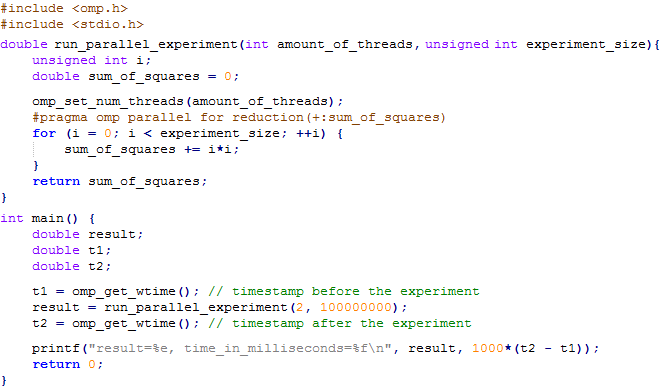
\includegraphics{source.png}
		\end{flushleft}		
		Для проведения сравнения данная программа запускалась для десяти значений experiment$\_$size (от $10^1$ до $10^9$ с шагом 111111110). Количество потоков (amount$\_$of$\_$threads) принималось равным 1 или 2.		
	\subsection{Описание операционной системы}
	Операционной системой для исследования была выбрана ОС Ubuntu (64-bit), запускаемая на 4х-ядерном компьютере с загрузочной флешки и на виртуальной машине с помощью программы Oracle VM VirtualBox, запущенной со следующими характеристиками:\\
		Оперативная память:	3152 Мб\\
		Процессоры:	4\\
		Порядок загрузки:	Гибкий диск, Оптический диск, Жесткий диск\\
		Ускорение:	VT-x/AMD-V, Nested Paging, PAE/NX, Паравиртуализация KVM\\
	\subsection{Сравнение}
	\subsubsection{График работы без виртуализации}
		\begin{figure}[h]
			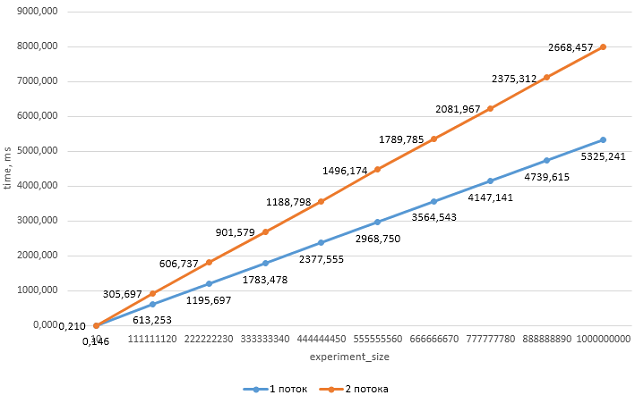
\includegraphics{withoutVirt.png}
			\label{ris:without}
		\end{figure}
		По данному графику видно, что в обоих случаях зависимость времени исполнения от количества потоков линейна. Работа двух параллельно работающих потоков осуществляется быстрее, кроме случая, когда значение experiment$\_$size мало.
\newpage
		\subsubsection{График работы с виртуализацией}
		\begin{figure}[h]
			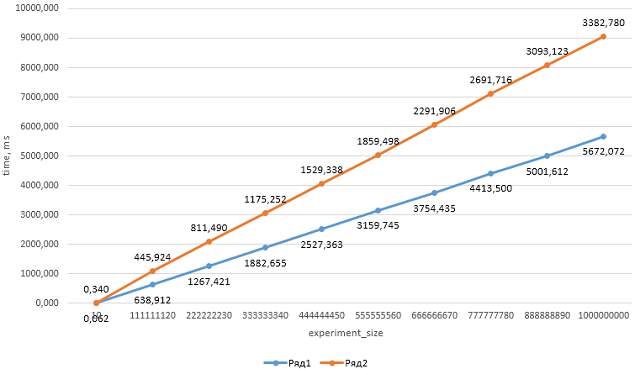
\includegraphics{withVirt.png}			
			\label{ris:with}
		\end{figure}
		По графику работы программы на виртуальной машине можно сделать такие же выводы, что и для работы программы без виртуализации. Так же следует заметить, что время работы для аналогичного количества потоков больше с виртуализацией, так как неизбежны растраты ресурсов на поддержание работы самой виртуальной машины.
\newpage
		\subsubsection{График ускорения}
		\begin{figure}[h]
			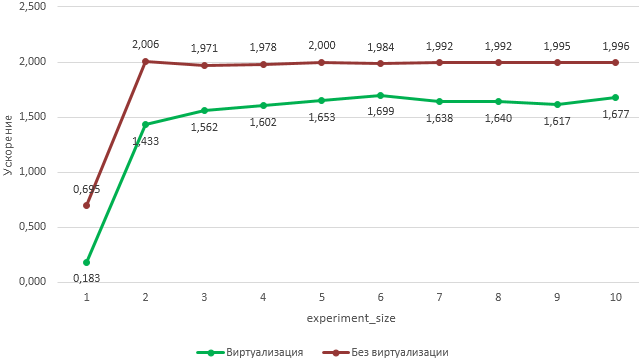
\includegraphics{acceleration.png}
			\label{ris:accel}
		\end{figure}
		По графику ускорений можно сделать следующие выводы:\\
		\begin{enumerate}
			\item Характер графиков ускорений для обоих случаев одинаков.
			\item Увеличение количества потоков сказывается лучше для работы программы без виртуализации.
			\item Начиная с некоторого значения, ускорение перестает изменяться.
			\item Ускорение программы без виртуализации более стабильно, не подвержено скачкам.
		\end{enumerate}
\newpage
\section{Выводы}
	\begin{itemize}
		\item Существует большой выбор иностранных материалов для изучения параллельных вычислений в системах с общей памятью, как платных, так и выложенных в свободный доступ.
		\item Выбор среди русскоязычных материалов меньше, однако достаточен для исследования данной тематики.
		\item Представлены только современные материалы, следовательно вся информация обновляется, не теряя актуальности.
		\item Выявлены различные критерии сравнения материалов, разной степени важности и достоверности, а также способы их вычисления. 
		\item Увеличение количества параллельных потоков ускоряет выполнение программы для немалых требуемых вычислениях.
		\item Работа программ при виртуализации проходит медленнее и меньше подвержена ускорению путем добавления дополнительных потоков, из-за затраты ресурсов на поддержание работы виртуальной машины.
	\end{itemize}

\newpage
\section{Используемые сайты}
	\begin{enumerate}
		\item \href{https://ru.wikibooks.org}{ru.wikibooks.org}
		\item \href{https://git-scm.com}{git-scm.com}
		\item \href{https://www.amazon.com}{Amazon.com}
		\item \href{https://www.ozon.ru}{ozon.ru}
		\item \href{https://scholar.google.ru/schhp?hl=ru&as_sdt=0,5}{Google Scholar}
		\item \href{http://arxiv.org}{arxiv.org}
		\item \href{http://www.journalmetrics.com}{journalmetrics.com}
		\item \href{https://computing.llnl.gov}{computing.llnl.gov}
		\item \href{https://www.tacc.utexas.edu}{tacc.utexas.edu}
		\item \href{http://freecomputerbooks.com}{freecomputerbooks.com}
		\item \href{http://www.freetechbooks.com}{freetechbooks.com}
		\item \href{https://www.elsevier.com/journals/title/all}{elsevier.com/journals}
		\item \href{http://www.sciencedirect.com}{sciencedirect.com}
		\item \href{https://www.computer.org}{computer.org}
		\item \href{http://ocw.mit.edu/index.htm}{ocw.mit.edu}
		\item \href{https://www.coursera.org}{coursera.org}
		\item \href{https://www.cs.berkeley.edu/}{cs.berkeley.edu}
		\item \href{https://www.coursetalk.com}{coursetalk.com}
		\item \href{http://soft.vub.ac.be/soft}{soft.vub.ac.be/soft}
		\item \href{https://books.google.ru}{books.google.ru}
		\item \href{http://elib.spbstu.ru}{elib.spbstu.ru}
		\item \href{http://scanlibs.com}{scanlibs.com}
		\item \href{http://pp-book.narod.ru}{pp-book.narod.ru}
		\item \href{https://www.lektorium.tv}{lektorium.tv}
		\item \href{http://www.hpcc.unn.ru}{hpcc.unn.ru}
		
	\end{enumerate}
\end{document}
